\documentclass[a4paper,11pt]{scrreprt}
\usepackage[utf8]{inputenc}
\usepackage[catalan]{babel}

\usepackage{listings}
\lstset{
  basicstyle=\sffamily,
  frame = lines
}

\usepackage{lscape}

\usepackage[load=abbr]{siunitx}
\sisetup{decimalsymbol=.,dp=0}

\usepackage{hyperref}
\hypersetup{colorlinks=true}

\usepackage{tikz}
\usetikzlibrary{arrows}
\usetikzlibrary{decorations.pathmorphing}
\usetikzlibrary{backgrounds}
\usetikzlibrary{positioning}
\usetikzlibrary{fit}
\usetikzlibrary{petri}
\usetikzlibrary{automata}
\usetikzlibrary{snakes}
\usetikzlibrary{shapes}
\usetikzlibrary{calc}
\usetikzlibrary{matrix}
\usepackage{circuitikz}
\usepackage{tikz-timing}

\title{ \LaTeX}
\subtitle{ Plantilla de \LaTeX}

\author{ ACatlla}
\date{ \today}


\begin{document}
\maketitle{}
\tableofcontents{}
\listoffigures{}

\chapter{Codi}
\label{chapter:codi}

\section{Codi Python}
\begin{lstlisting}[language=python]
def a():
   print "Hola!"
\end{lstlisting}

\section{Codi Python importat}
\lstinputlisting[language=python]{codi_python.py}

\section{Codi C importat}
\lstinputlisting[language=c]{codi_c.c}

\section{Codi Python entre text}
Podem afegir codi \lstinline[language=python]!def a(b):! entre text.


\chapter{Enllaços}
\section{Enllaços entre elements del document}
\begin{itemize}
\item Enllaç al capítol de codi, capítol \ref{chapter:codi}
\item Enllaç al capítol de codi, \href{chapter:codi}{Codi}
\end{itemize}

\section{Enllaços a altres documents PDF}
Enllaç a document PDF extern, \href{graf}{màquina d'estats}

\section{Enllaços web}
Enllaç a una web \href{ocw.itic.cat}{OCW iTIC}

\chapter{ Taules}
\section{Taules mòbils}
La taula corresponent és la taula \ref{tab:taula1} que es situa en la posició del text que correspon a la millor ubicació segons l'algoritme. 
És una taula mòbil centrada, que ajusta la seva amplada a l'amplada de la pàgina. Consta de tres columnes, la primera amb els elements tabulats a l'esquerre, la segona amb els elements tabulats al centre i la tercera amb els elements tabulats a la dreta. No consta de línies laterals. A l'apartat \ref{taules fixes} podrem veure taules fixes clicant a la referència.

\begin{table}[tbh]
  \centering
  \begin{tabular}{l|c|r}%primer elem tabulat a l'esquerra, segon tabulat al centre i tecer tabulat a la dreta i línies verticals entre mig
    \hline % línia horitzontal per separació
    \textbf{Capcelera c1}  & \textbf{Capcelera c3}  & \textbf{Capcelera de la c2} \\
    \hline
    element f1 c1  & element f1 c2  & element f1 c3 \\
    element f2 c1  & element f2 c2  & element f2 c3 \\
    \hline
  \end{tabular}
  \caption{Explicació de la taula}
  \label{tab:taula1}
\end{table}


\section{Taules fixes}
Taula amb quatre columnes tabulades a l'esquerre, les quals tenen una capcelera compartida entre dues columnes i la columna 4 no té capcelera.

\label{taules fixes}
\begin{center}
  \resizebox{\textwidth}{!}{ %
  \begin{tabular}{|l|l|l|l|}
    \hline
    \multicolumn{2}{|c|}{\textbf{Capcelera comú de la columna 1 i 2}} & \textbf{Capcelera de la columna3}& \\    
    \hline
    element f1 c1  & element f1 c2  & element f1 c3 & element f1 c4 \\
    element f2 c1  & element f2 c2  & element f2 c3 & element f2 c4 \\
    \hline
  \end{tabular}
  }
\end{center}

\chapter{Figures}
\section{Figures mòbils}
La taula corresponent és la figura \ref{fig:osci} que es situa en la possició del text que correspon a la millo ubicació segons l'algoritme.
\begin{figure}[h]
  \centering
  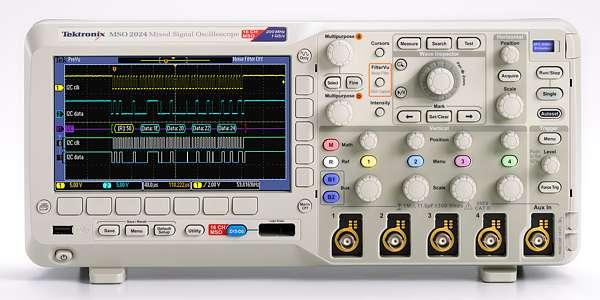
\includegraphics[width=0.5\textwidth]{osci.jpg}
  \caption{Explicació de la figura}
  \label{fig:osci}
\end{figure}

\section{Figures fixes}
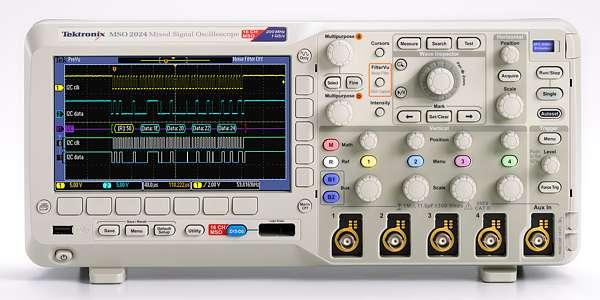
\includegraphics[width=0.75\textwidth]{osci.jpg}


\chapter{ Matemàtiques}

\section{Símbols matemàtics}

Símbol de sumatori $\sum_{inici}^{fi} eq.$ \\

Integral $\int_{inici}^{fi} eq.$\\

Fracció $\frac{numerador}{denominador}$\\

Símbol de la derivada $\partial$ \\

Símbol més, menys $\pm$

\section{Representació de funcions}
\subsection{Representació de funcions matemàtiques entre text}

Escribim text i entremig si volem posar una funció matemàtica $E=mc^2$ per exemple.

\subsection{Representació de les funcions matematiques independients}
\begin{itemize}
\item En cas de que volguem posar l'equació a part ho farem de la següent manera:
\begin{equation}
x=\frac{-b\pm\sqrt{b^2 - 4ac}}{2a}
\end{equation}
\item En cas de que volguem fer una resolució d'una equació
\begin{eqnarray*}
  \label{eq:fonamental}
  F(x) &=& x ( x^3 -2x - 1) \\
       &=& x^4 - 2x^2 - x \\
\end{eqnarray*}
\end{itemize}

\chapter{Circuits}
\begin{center}
  \begin{circuitikz}[scale=0.75]
    \draw 
    (0,0) node[op amp,yscale=-0.77] (opamp2) {}
    (opamp2.+) node[above] {$v_+$}
    (opamp2.-) node[above] {$v_-$}
    (opamp2.+) -- (-2,0.5)
    (opamp2.-) -- (-2,-0.5)
    (opamp2.out) -- (2,0);
    \draw
    (-8,0) node[ocirc]{} 
           node[left]{$V_{in}$}
    (-8,0) to [C=470n] (-5,0)
    (-5,0.5) -- (-5,-0.5) 
    (-5,0.5) to [R=10k] (-2,0.5)
    (-2,-0.5) to [R=10k] (-5,-0.5)
    (-2,0.5) -- (-2,2)
    to [R=10k] (2,2)
    -- (2,0)
    -- (3,0)
    node[ocirc]{}
    node[right]{$V_o$}
    (-2,-4.5) to [cspst] (-2,-0.5) 
    (-2,-4.5) node[ground]{};
    \draw 
    (-4,-2.5) node[op amp,yscale=-0.77] (opamp1) {}
    (opamp1.+) node[above] {$v_+$}
    (opamp1.-) node[above] {$v_-$}
    (opamp1.+) -- (-6,-2)
    -- (-8,-2)
    node[ocirc]{}
    node[left]{$clk$}
    (opamp1.-) -- (-6,-3)
    -- (-6,-4.5)
    node[ground]{};
    \draw[-latex]
    (opamp1.out) -- (-2.25,-2.5);
  \end{circuitikz}
\end{center}

\chapter{Diagrames}
\section{Diagrames de blocs}
\begin{center}
  \begin{tikzpicture}[auto,>=latex']
    \tikzstyle{block} = [draw, shape=rectangle, minimum height=3em, minimum width=3em, node distance=2.75cm, line width=1pt]
    \tikzstyle{io} = [draw=none, fill=none, shape=circle, minimum height=3em, minimum width=3em, node distance=3cm, line width=1pt]
    \tikzstyle{clk} = [draw=none, fill=none, shape=circle, minimum height=3em, minimum width=3em, node distance=2cm, line width=1pt]
    %Creating Blocks and Connection Nodes
    \node [io, text width=1.5cm](input) {Senyal original};
    \node [block, right of=input,text width=2.25cm] (m0) {Multiplicador 0 i 1};
    \node [clk, above of=m0](clk0) {$clk_0$};
    \node [block, right of=m0, text width=1.25cm] (bp) {Pas banda};
    \node [block, right of=bp] (amp0) {Amplificador};
    \node [block, right of=amp0] (tx) {Tx};
    \node [block, below of=tx] (rx) {Rx};
    \node [block, left of=rx] (amp1) {Amplificador};
    \node [block, left of=amp1,text width=2.25cm] (m1) {Multiplicador -1 i 1};
    \node [clk, below of=m1](clk1) {$clk_1$};
    \node [block, left of=m1, text width=1.125cm] (lp) {Pas baix};
    \node [io, left of=lp, text width=1.25cm] (output) {Senyal sortida};
    %Conecting Blocks
    \begin{scope}[line width=1pt]
         \draw[->] (input) -- (m0);
         \draw[->] (clk0) -- (m0);
         \draw[->] (m0) -- (bp);
         \draw[->] (bp) -- (amp0);
         \draw[->] (amp0) -- (tx);
         \draw[snake=expanding waves, segment angle=30] (tx) -- (rx);
         \draw[->] (rx) -- (amp1);
         \draw[->] (amp1) -- (m1);
         \draw[->] (clk1) -- (m1);
         \draw[->] (m1) -- (lp);
         \draw[->] (lp) -- (output);
    \end{scope}

  \end{tikzpicture}
\end{center}

\section{Diagrames d'estats}
\begin{tikzpicture}[shorten >=1pt,node distance=5cm,on grid,>=stealth',auto]
\node[state,initial]  (e_0)                      {Repós};
\node[state]          (e_1) [ right=of e_0][text width=2.25cm]{Estat alt $B=1->sc$ $B=0->s$};
\node[state]          (e_2) [ right=of e_1][text width=2.25cm]{Estat baix $B=1->r$ $B=0->p$};
\path[->,font=\scriptsize] 
          (e_0) edge  [bend left] node        {flag up}  (e_1)
          (e_1) edge  [bend left] node        {flag down}  (e_2)
                edge  [bend left] node        {$B=1$} (e_0)
          (e_2) edge  [bend left] node        {flag up}  (e_1)
                edge  [bend left] node        {$A=1$} (e_0);
\end{tikzpicture}

\begin{landscape}
\begin{figure}[!h]
  \centering
  \begin{tikzpicture}[shorten >=1pt,node distance=2.5cm,on grid,>=stealth',auto]

    \tikzstyle{bigbox} = [draw=blue!50, thick, fill=blue!10, rounded corners, rectangle]
    \tikzstyle{bigbox1} = [draw=green!50, thick, fill=green!10, rounded corners, rectangle]

    \node[state]  (main) {main};

    \node[state]  (automat) [below = of main]{automat};
    \node[state]  (menu) [left = of automat] {menu};
    \node[state]  (controller) [right = of automat]{controller};

    \node[state]  (tools) [below = of automat] {tools};
    \node[state]  (print) [below left = of menu] {print};

    \node[state]  (time) [below = of tools]{time};
    \node[state]  (lcd) [right = of time] {lcd};
    \node[state]  (sensor) [right = of lcd] {sensor};

    \node[state]  (rtc) [below = of time] {rtc};
    \node[state]  (display) [right = of rtc] {display}; 
    \node[state]  (accel) [right = of display] {accel};  

    \node[state]  (buzzer) [left = of rtc] {buzzer};
    \node[state]  (led) [left = of buzzer] {led};

    \node[state]  (twi) [below = of display] {twi};

    \node[state]  (botons) [left = of led] {botons};
    \node[state]  (polsador) [left = of botons] {polsador};

    \node[state]  (interrup) [below = of buzzer] {interrup};

    \node[state]  (esdv) [right = of sensor] {esdv};
    \node[state]  (queue) [right = of esdv] {queue};

%    \node[state]  (timer) [left = of display] {timer};
%    \node[state]  (serial) {serial};

\begin{pgfonlayer}{background}
  \node[bigbox] [fit = (display) (rtc) (accel)] (display_rtc_accel) {};
  \node[bigbox] [fit = (lcd) (time) (sensor)] (lcd_time_sensor) {};
  \node[bigbox] [fit = (botons) (polsador)] (botons_polsador) {};
  \node[bigbox1] [fit = (buzzer) (led)] (buzzer_led) {};
  \node[bigbox] [fit = (queue) (esdv)] (queue_esdv) {};
  \node[bigbox1] [fit = (menu) (automat) (controller) (print) (tools) ] (timer) {};
  \node[bigbox1] [fit = (lcd)] (timer1) {};
  \node[bigbox] [fit = (menu) (automat) (controller)] (menu_automat_controller) {};
\end{pgfonlayer}

    \path[<->,font=\scriptsize] 
    (automat) edge node {} (menu)
              edge node {} (controller)
    ;
    \path[->,font=\scriptsize] 
    (automat) edge node {} (main)
    (tools) edge node {} (automat)
            edge node {} (menu)
    (print) edge node {} (menu)

    (lcd_time_sensor) edge node {} (tools)
                      edge node {} (print)

    (lcd) edge node {} (automat)
    (sensor) edge node {} (controller)

    (display) edge node {} (lcd)
    (rtc) edge node {} (time)
    (accel) edge node {} (sensor)

    (interrup) edge node {} (rtc)

    (botons_polsador) edge node {} (automat)
    (buzzer_led) edge node {} (tools)
    ;
    \path[dashed,->,font=\scriptsize] 
    (queue_esdv) edge node {} (menu_automat_controller)
    (twi) edge node {} (display_rtc_accel)
    (interrup) edge node {} (botons_polsador)
    ;
   \end{tikzpicture}
  \caption{Esquema dels mòduls software.}
  \label{fig:esquema_bloc_software}
\end{figure}
\end{landscape}

\begin{figure}[!h]
  \begin{tikzpicture}[font=\ttfamily,node distance=0.75cm,
    mymatrix/.style={matrix of nodes, nodes=typetag, row sep=1em},
    mycontainer/.style={draw=gray, inner sep=1ex},
    typetag/.style={draw=gray, inner sep=1ex, anchor=west},
    title/.style={draw=none, color=gray, inner sep=0pt}
    ]
    \matrix[mymatrix] (mx1) {
      |[title]|Alimentació \\
      Bateria \\
      Càrrega \\
    };
    \matrix[mymatrix, right=of mx1.north east, matrix anchor=north west] (mx2) {
      |[title]|Interacció \\
      Botonera \\
      Display \\
    };
    \matrix[mymatrix, right=of mx2.north east, matrix anchor=north west] (mx3) {
      |[title]|Avisadors \\
      LED \\
      Buzzer \\
    };
    \matrix[mymatrix, right=of mx3.north east, matrix anchor=north west] (mx4) {
      Microcontrolador \\
      Acceleròmetre \\
      Memòria \\
    };
    \matrix[mymatrix, right=of mx4.north east, matrix anchor=north west] (mx5) {
      RTC \\
      RF\\
    };
    \node[mycontainer, fit=(mx1)] {};
    \node[mycontainer, fit=(mx2)] {};
    \node[mycontainer, fit=(mx3)] {};
    
  \end{tikzpicture}
  \caption{Esquema general del muntatge.}
  \label{fig:esquema_bloc}
\end{figure}




\chapter{Dibuixos}

\begin{center}
\begin{tikzpicture}[line width=1.25pt]
  \draw[<->,line width=1.5pt] (-6.5,0) -- (6.5,0) node[right] {$f$};
  \draw[->,line width=1.5pt] (0,-0.2) -- (0,1.5) node[above] {};

  \coordinate (o) at (0,0);
  \coordinate (on) at (0,0);

  \coordinate (b) at ($(o)+(0.125,0)$);
  \coordinate (c) at ($(o)+(0.5,1)$);
  \coordinate (a) at ($(o)+(1.5,0)$);
  \draw (b) -- (c) -- (a);

  \coordinate (bn) at ($(on)+(-0.125,0)$);
  \coordinate (cn) at ($(on)+(-0.5,1)$);
  \coordinate (an) at ($(on)+(-1.5,0)$);
  \draw (bn) -- (cn) -- (an);

  \draw ($(o)+(0.5,0.1)$) -- ($(o)+(0.5,0)$) node[below] {$f_c$};
  \draw ($(on)+(-0.5,0.1)$) -- ($(on)+(-0.5,0)$) node[below] {$f_c$};

\end{tikzpicture}
\end{center}

\begin{center}
\begin{tikzpicture}[line width=1.25pt]
  \draw[<->,line width=1.5pt] (-6.5,0) -- (6.5,0) node[right] {$f$};
  \draw[->,line width=1.5pt] (0,-0.2) -- (0,1.5) node[above] {};

  \coordinate (od) at (4,0);
  \coordinate (odn) at (-4,0);
  \draw[->] ($(od)+(0,0)$) -- ($(od)+(0,1)$);
  \draw[->] ($(odn)+(0,0)$) -- ($(odn)+(0,1)$);
  \draw ($(od)+(0,0)$) node[below] {$f_s$};
  \draw ($(odn)+(0,0)$) node[below] {$f_s$};
\end{tikzpicture}
\end{center}


\begin{center}
\begin{tikzpicture}[line width=1.25pt,scale=1]
  \draw[<->,line width=1.5pt] (-6.5,0) -- (6.5,0) node[right] {$f$};
  \draw[->,line width=1.5pt] (0,-0.2) -- (0,1.5) node[above] {};

  \coordinate (o) at (4,0);
  \coordinate (on) at (4,0);

  \coordinate (b) at ($(o)+(0.125,0)$);
  \coordinate (c) at ($(o)+(0.5,0.5)$);
  \coordinate (a) at ($(o)+(1.5,0)$);
  \draw (b) -- (c) -- (a);

  \coordinate (bn) at ($(on)+(-0.125,0)$);
  \coordinate (cn) at ($(on)+(-0.5,0.5)$);
  \coordinate (an) at ($(on)+(-1.5,0)$);
  \draw (bn) -- (cn) -- (an);

  \draw ($(o)+(0,0.1)$) -- ($(o)+(0,0)$) node[below] {$f_s$};
  \draw ($(o)+(0.5,0.1)$) -- ($(o)+(0.5,0)$) node[below] {$f_u$};

  \coordinate (o) at (-4,0);
  \coordinate (on) at (-4,0);

  \coordinate (b) at ($(o)+(0.125,0)$);
  \coordinate (c) at ($(o)+(0.5,0.5)$);
  \coordinate (a) at ($(o)+(1.5,0)$);
  \draw (b) -- (c) -- (a);

  \coordinate (bn) at ($(on)+(-0.125,0)$);
  \coordinate (cn) at ($(on)+(-0.5,0.5)$);
  \coordinate (an) at ($(on)+(-1.5,0)$);
  \draw (bn) -- (cn) -- (an);

  \draw ($(on)+(0,0.1)$) -- ($(o)+(0,0)$) node[below] {$f_s$};
  \draw ($(on)+(-0.5,0.1)$) -- ($(on)+(-0.5,0)$) node[below] {$f_u$};
\end{tikzpicture}
\end{center}


\chapter{Timmings}

\tikztimingmetachar{Y}{8{U}}
\tikztimingmetachar{G}{6{L}}
\tikztimingmetachar{P}{3{U}}
\tikztimingmetachar{F}{3{D}}

\begin{center}
\begin{tikztimingtable}
  \texttiming{T 3{YG} U}\\
  \texttiming{T 7{PF} U}\\
  \\
  \extracode
  \begin{pgfonlayer}{background}
    \begin{scope}[semitransparent,semithick]
      \vertlines{-2,-8,-16,-22,-30,-36,-44}
    \end{scope}
  \end{pgfonlayer}

\end{tikztimingtable}
\end{center}



\begin{tikzpicture}[timing/picture,thick,scale=1,line width=0.5pt]

  \draw (5,3) node [above] {\footnotesize{40ms}};
  \draw (12,3) node [above] {\footnotesize{30ms}};
  \draw (2.5,-3) node [below] {\footnotesize{15ms}};
  \draw (5.5,-3) node [below] {\footnotesize{15ms}};
 
  \draw[<->] (1.05,3) -- (8.95,3);
  \draw[<->] (9.05,3) -- (14.95,3);
  \draw[-] (1,3.5) -- (1,-3.5);
  \draw[-] (9,3.5) -- (9,-3.5);
  \draw[-] (15,3.5) -- (15,-3.5);
  \draw[-] (23,3.5) -- (23,-3.5);
  \draw[-] (29,3.5) -- (29,-3.5);
  \draw[-] (37,3.5) -- (37,-3.5);
  \draw[-] (43,3.5) -- (43,-3.5);

  \draw[<->] (1,-3) -- (3.95,-3);
  \draw[<->] (4.05,-3) -- (6.95,-3);
  \draw[-] (4,0) -- (4,-3.5);
  \draw[-] (7,0) -- (7,-3.5);

  \timing at (0,1){T 3{YG} U};
  \timing at (0,-1) {T 7{PF} U};
\end{tikzpicture}

\tikztimingmetachar{Y}{8{U}}
\tikztimingmetachar{G}{8{L}}
\tikztimingmetachar{P}{4{U}}
\tikztimingmetachar{F}{4{D}}

\begin{center}
\begin{tikzpicture}[timing/picture,thick,scale=1,line width=0.5pt]

  \draw (5,3) node [above] {\footnotesize{40ms}};
  \draw (13,3) node [above] {\footnotesize{40ms}};
  \draw (3,-3) node [below] {\footnotesize{20ms}};
  \draw (7,-3) node [below] {\footnotesize{20ms}};
 
  \draw[<->] (1.05,3) -- (8.95,3);
  \draw[<->] (9.05,3) -- (16.95,3);
  \draw[-] (1,3.5) -- (1,-3.5);
  \draw[-] (9,3.5) -- (9,-3.5);
  \draw[-] (17,3.5) -- (17,-3.5);
  \draw[-] (25,3.5) -- (25,-3.5);
  \draw[-] (33,3.5) -- (33,-3.5);
  \draw[-] (41,3.5) -- (41,-3.5);
  \draw[-] (49,3.5) -- (49,-3.5);

  \draw[<->] (1,-3) -- (4.95,-3);
  \draw[<->] (5.05,-3) -- (8.95,-3);
  \draw[-] (5,0) -- (5,-3.5);

  \timing at (0,1){T 3{YG} U};
  \timing at (0,-1) {T 6{PF} U};
\end{tikzpicture}
\end{center}

\begin{center}
\begin{tikzpicture}[timing/picture,thick,scale=1,line width=0.5pt]
  \draw[-] (1,3.5) -- (1,-3.5);
  \draw[-] (9,3.5) -- (9,-3.5);
  \draw[-] (17,3.5) -- (17,-3.5);
  \draw[-] (25,3.5) -- (25,-3.5);
  \draw[-] (33,3.5) -- (33,-3.5);
  \draw[-] (41,3.5) -- (41,-3.5);
  \draw[-] (49,3.5) -- (49,-3.5);

  \timing at (0,1){T 3{YG} U};
  \timing at (0,-1) { 3{D} 5{PF} 4{U} 3{D}};
\end{tikzpicture}
\end{center}

\chapter{Definir comandes}

\newcommand{\exCom}{\textsl{Exemple comanda}}

Podem utilitzar la comanda definida \exCom{}

\newcommand{\vect}[1]{(#1_1,#1_2,\dots,#1_n)}

Nova comanda amb arguments, $\vect{a}$
\chapter{Entorns}

\NewDocumentEnvironment{component}{m}%
{
  \begin{minipage}[b]{0.6\linewidth}
    \small
}{
  \end{minipage}
  \hfill
  \includegraphics[width=0.3\linewidth]{#1}
  \par
}

\begin{component}{osci.jpg}
  \begin{itemize}
  \item   Descripció d'un copmonent.   Descripció d'un copmonent.
  \item   Descripció d'un copmonent.   Descripció d'un copmonent.
  \item   Descripció d'un copmonent.   Descripció d'un copmonent.
  \end{itemize}
\end{component}

\end{document}

